% status: 0
% chapter: Data

\title{IBM Big Replicate}


\author{Manoj Joshi}
\affiliation{%
  \institution{Indiana University}
 \streetaddress{School of Informatics, Computing, and Engineering}
  \city{Bloomington}
  \state{IN}
  \postcode{47408}
  \country{USA}}
\email{manjoshi@iu.edu}

% The default list of authors is too long for headers}
\renewcommand{\shortauthors}{Manoj}


\begin{abstract}
As organizations grow, the amount of data they store grows exponentially. The 
data is essentially stored in multiple data centres across various regions. 
Since there is continuous communication between data centres, reliability and 
availability of data centres are the key factors for any organization to store 
data. A disaster at a data centre might prove to be really expensive for many 
organizations since it would hamper the communication between data centres. To 
solve this problem of losing data in large data centres, IBM provides IBM Big
Replicate as a solution which is an Enterprise-class active-active data 
replication solution for Hadoop and object stores.
\end{abstract}

\keywords{hid-sp18-408, IBM Big Replicate, Data Replication, WANdisco Fusion}


\maketitle

\section{Introduction}

Many organizations prefer Hadoop over the traditional data warehouse solutions
because of the cost. However, industry experts have some concerns that Hadoop is
not reliable enough as the database technologies. Few of the concerns of Hadoop
are:
\begin{enumerate}
\item \textbf{Backup reliability and data  consistency across clusters and
locations:} Backup and Replication in Hadoop is based on distributed copy which 
is designed for copying only the files and does not provide replication of the
entire cluster.
\item \textbf{Performance in distributed environments:} Since there is no
consistency across locations, applications would return different results
depending on which region they run. If data is inconsistent or if the data is
out-of-date, it would introduce business risk which might incur huge costs. 
Since business decisions are taken on data, consistency should be present in 
data across all the locations. 
\item \textbf{Meeting application service-level-agreements:} The deployment of
real-time solutions with stringent service-level-agreement and high computing
power such as analytical solutions would be a difficult task. 
\item \textbf{On-premise IT costs:} Often, organizations would need to come up
with solutions to reduce costs for on-premise infrastructure. They need to find
solutions to expand the infrastructure as and when needed in order to avoid 
costs. The cloud is one way to dynamically expand the infrastructure
\end{enumerate}
IBM Big Replicate helps the organizations ensure business continuity by
providing real-time replication of data between multiple Hadoop clusters with 
zero recovery point objective (RPO) and recovery time objective (RTO). The
replication engine provides automated data recovery and synchronization across 
various regions.  IBM Big Replicate is flexible in a way that it supports 
replication across different Hadoop distributions and object stores
~\cite{hid-sp18-408-IBMBigReplicate-intro}.

\section{Architecture}

There are two main components in the IBM Big Replicate - Fusion servers and IHC 
servers. The Fusion servers acts as a proxy for systems that write into the 
HDFS. It also writes replicated data into the local file system. There can be 
multiple Fusion servers in the IBM Big Replicate system. On the other hand, the 
IHC servers read from the file system and transfer the data to other clusters.
Although the architecture diagram Figure~\ref{f:architecture} shows only two 
clusters in a data center, in practice there can be multiple clusters in each 
data center. The labels on the lines in Figure~\ref{f:architecture} indicate the
purpose and also the direction of flow of data. IHC servers read data from the 
file system and Fusion servers write into it. Since the Fusion servers write
data into the file system, coordination takes place between the Fusion servers.
IBM Big Replicate is an active-active replication system wherein each cluster or
a data center as a whole has access to replicated copy of the complete data in 
real time. This way, a cluster or datacenter can obtain updated data from any 
replicated HDFS. As the number of connections between clusters is very minimal,
it makes the network security and management easier. The workflow of IBM Big 
Replicate is as follows:
First, the application makes a request to create a file. The fusion coordinates 
the file open operation to other clusters involved. Then, file is added to the 
underlying storage. Following this, the IHC server gets the data from the 
cluster and sends the data to remote clusters. Lastly, the Fusion server 
coordinates the file close operation to other clusters involved 
~\cite{hid-sp18-408-IBMBigReplicate-architecture}.

\begin{figure}[!ht]
  \centering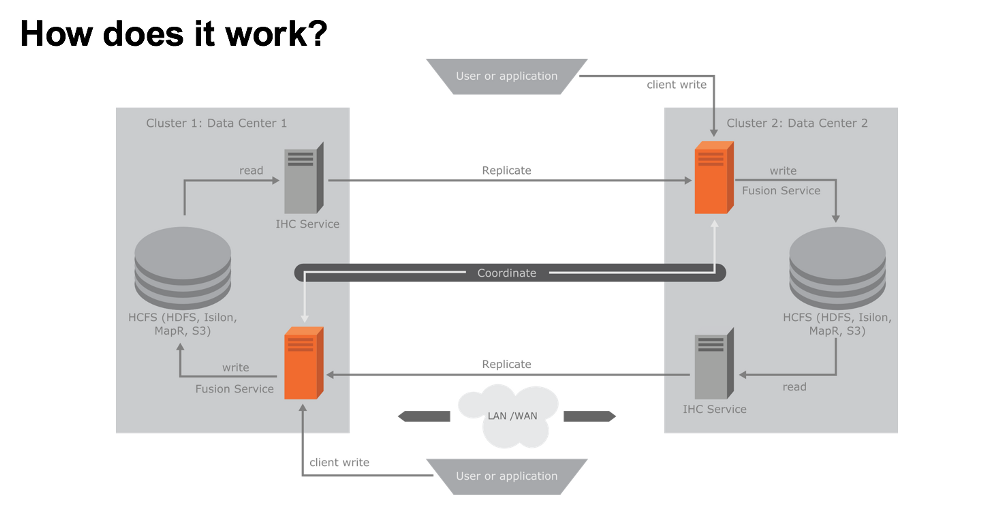
\includegraphics[width=\columnwidth]
  {image/IBM-Replicate-Architecture.png}
  \caption{IBM Big Replicate Architecture
  ~\cite{hid-sp18-408-IBMBigReplicate-architecture}}\label{f:architecture}
\end{figure}

\section{Features}

IBM Big Replicate provides replication for on-premise systems and also for 
cloud systems. The important features are:

\subsection{100 percent availability}
There is no significant administrative overhead involved in setting up,
monitoring, maintenance and disaster recovery of the data center. It does not
need manual intervention as replication happens in such a way that data
consistency is guaranteed across the clusters. It supports any Hadoop
distributions running across the clusters and the data centers. Lastly, since
the data replication happens in real time, scheduled backup of data after the 
normal business hours is not necessary.

\subsection{Continuous replication and migration}
There is no migration downtime as source and target operate parallely during 
migration process. There is no heavy overhead involved in data transfer since
the directories are scanned periodically and are done in batches. To support 
scalability, IBM Big Replicate does not limit the number of servers and data
centers.

\subsection{Replicate anything}
New plugins can be developed to extend the WANdisco Fusion to incorporate new
data sources. The Fusion components can be reused for bandwidth management,
encryption key handling and also licensing. The SDK can be used to customize
the Fusion UI for the new plugins to provide your own user interface. Once the 
Fusion UI has been developed, it can be used to support generic functionality.

\subsection{Cloud migration and hybrid cloud}
IBM Big Replicate can be used to integrate on-premise Hadoop clusters with 
Amazon AWS Data Lake with WANdisco Fusion and Amazon S3. Data can be moved
between any Fusion based on-premise setup and Amazon S3. The system setup is
simple in both on-premise and Amazon environment. This is possible using the 
AWS Cloud Formation templates. To monitor the setup, IBM Big Replicate provides
admin console which also handles scheduling and audit. An EMR cluster could be
setup referencing the data that is currently being replicated into Amazon S3.
This serves as a low cost disaster recovery environment. Lastly, IBM Big 
Replicate also supports data replication between different cloud vendors who
support Fusion such as Microsoft Azure, IBM OpenStack Swift and Google Cloud.

\subsection{Bulk transfer of changing data}
Data can be written to Amazon AWS Snowball using the same API which is being
used to interact with Amazon S3. Storage on Amazon AWS Snowball can be leveraged
without experiencing delays over the network. Since data is replicated 
continuously, recovery can be done network or system failures automatically.

\subsection{Data Replication on Google Cloud}
IBM Big Replicate uses the Google Platform Templates and makes it easy to set up
Google cloud environment with replication. It provides a console for monitoring,
scheduling and to audit the cloud resources. It facilitates movement of data
between Fusion supported environment and Google Cloud. Because of this, data can
be moved from Google Cloud and other cloud environments like Microsoft Azure,
IBM Openstack Swift and Amazon S3.

\subsection{Data Replication on Microsoft Azure HDInsight}
The WANdisco Fusion can be added to the Azure HDInsight cluster in a single
click installation from within Azure marketplace to provide replication of data
at scale between various cloud environments. The Fusion server does not require
dedicated data storage systems which leads to a better cost savings along with 
the return on investment. The administrator can select subsets of data for
replication which gives control to the administrator to figure out where the 
data will reside.

\subsection{Data Replication on Microsoft Azure Data Box}
Data can be replicated in Azure Box by using the same API that is used to
interact with Azure Cloud. This allows the client to take advantage of storage
on existing Azure Data box without delays over network.

\subsection{Data Replication on Oracle BDA and Oracle BDCS}
IBM Big Replicate can be deployed in environments which run any mix of various 
HCFS compatible distributions. This eliminates the need for intervention for 
out-of-sync conditions. Data replication happens across any geographic distance
and across various data centers running Hadoop. Since many organizations run
Oracle BDA and BDCS, cost of data migration is greatly reduced by the use of 
IBM Big Replicate.


\subsection{Data Replication on IBM Openstack Swift}
The setup is simple for both on-premise and IBM cloud based environments. This
Set up can be easily achieved using IBM Openstack Swift. Installation can be 
done using the standard cloud vendor utilities. Data can be moved between Fusion
supported on-premise environment and IBM Openstack Swift. Since IBM Openstack
Swift cloud environment is based on Fusion, data can be moved between other
cloud environments like Microsoft Azure, Amaozon S3 and Google Cloud
~\cite{hid-sp18-408-IBMBigReplicate-features}.

\section{Use Cases}
IBM Big Replicate supports data replication in various domains. The most 
prominent use cases are:

\subsection{Financial industry}
The main challenge faced by the financial industry is the inconsistency of data
across various clusters and data centers. This introduces a business risk in 
distributed environments. If business decisions are not done on updated data,
the service level agreements are not met. The solution provided by IBM Big
Replicate includes continuous availability of consistent data across regions, 
multi-data center data ingestion enabling real-time business decisions across
regions, elimination of underutilized servers for backup which saves huge amount
of hardware costs, replication of selected data across regions to avoid movement
of sensitive information which would otherwise pose a data security threat, 
incorporating multi vendor cloud solutions to effectively manage costs according
to business needs.

\subsection{Telecommunications industry}
The telecommunication industry faces a challenge of consistent data replication
across multiple data centers. Each data center would receive terabytes of raw
data everyday. The velocity with which the data moves is the main reason for not
having effective data backup and recovery strategy. So the data backup has to be
done outside of normal business hours increasing the costs involved. The
solution provided by IBM Big Replicate includes improved data availability 
where, only the vital data is replicated continuously and made available to
other clusters. Since vital data is transferred in real-time, data transfer load
is heavily reduced for after business hours. Lastly, since the active-active
replication strategy replicates data in real-time, it simplifies the data flow
by avoiding intermediate connections between network elements.

\subsection{Utilities industry}
The utilities industry is faced with a challenge when different data streams are
brought online. Ingestion of all the data into a single cluster is not feasible.
The data lakes become complicated and new pipelines have to be setup to transfer
data between the clusters. The IBM Big replicate includes automatic restoration
of systems in minutes after a failure occurs. Because of this feature, data 
streams can be brought online instantaneously. Once online, these data stream
resources could be utilized effectively and the existence of multiple data 
streams online would enable load balancing. It also improves the performance
of the cluster by continuously replicating data without any overhead. Lastly,
data analysis can be done in real-time since data is ingested and processed on 
all clusters immediately.

\subsection{Insurance industry}
The insurance industry keeps updating their policies every often. Due to this, a
significant amount of time is spent on policy updation, maintenance and
monitoring. It requires a lot of manual intervention to handle out-of-sync 
conditions. Sharing resources among production clusters might affect the overall
performance since a policy maybe applied only on a subset of data and not 
throughout. Using the IBM Big Replicate solution, data is made available when 
and where it’s needed, and automatically re-synchronizes as the network
bandwidth allows. The solution makes every backup server fully writable as well
as readable and facilitates sharing of subset of data across regions or data 
centers. The selective replication on a per-folder basis allows the 
administrators to define the way in which data has to replicated across regions
based on the policies. Data security risks are reduced by working with all the 
network encryption methods available for Hadoop. The only requirement is that
the servers should be exposed through the firewall for data replication between
the data centers on the premise and the cloud
~\cite{hid-sp18-408-IBMBigReplicate-intro}.

\section{Conclusion}
A large number of organizations adopt the Hadoop ecosystem to store data
efficiently. The reliability of a system has to be really high if the data is
large and the data is used to make business rules. For the system to have high
reliability and up-time, an efficient data backup strategy has to be adopted. To
incorporate the business costs involved in data replication and migration, the
data backup strategy has to replicate data in real-time. Considering these
factors, IBM Big Replicate is a simple yet flexible data replication solution 
that supports data replication for on-premise and cloud based environments. 
The most important advantage of using IBM Big Replicate is that it reduces the
resource allocation for data replication after business hours and thereby 
reduces the overall cost.

\begin{acks}

  The author would like to thank Dr.~Gregor~von~Laszewski for his
  support and suggestions to write this paper.

\end{acks}

\bibliographystyle{ACM-Reference-Format}
\bibliography{report} 


